\documentclass{article}
\usepackage[utf8]{inputenc}

\usepackage{hyperref}
\usepackage{graphicx}
\usepackage{subcaption}
\usepackage{float}
\usepackage{amsmath}
\usepackage{amssymb}
\usepackage{setspace}
\usepackage{xfrac}
\usepackage{eufrak}
\usepackage{indentfirst}
\usepackage{tikz}
\usepackage{physics}

\title{ECE329 Final Review Solutions - Cramming Carnival}
\author{Author: Members of HKN}
\date{}

% \newcommand{\dd}[1]{\mathrm{d}#1}

\usepackage[makeroom]{cancel}
\usepackage[letterpaper, portrait, margin=1in]{geometry}
\usepackage{graphicx}
\usepackage{float}
\usepackage{xcolor}

\pagenumbering{arabic}

\begin{document}

\maketitle

\section{Mundane Multiline}

\begin{figure}[h]
\begin{center}
    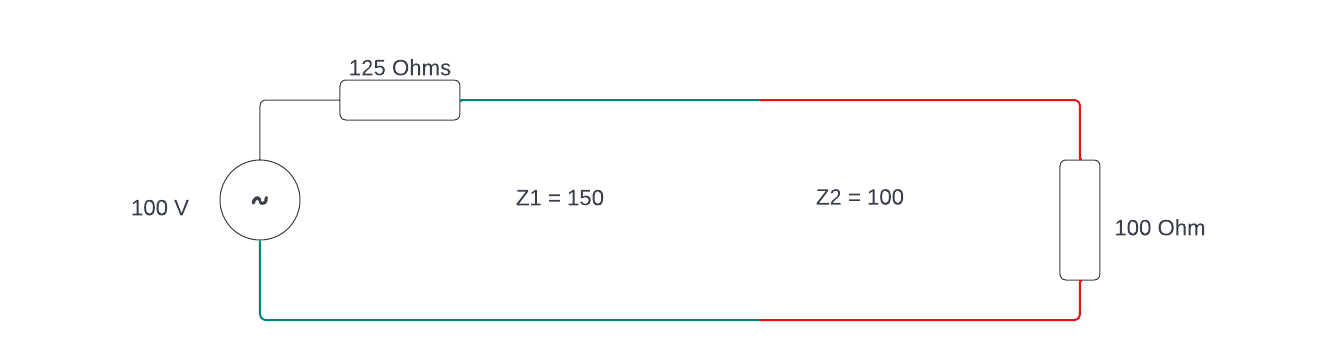
\includegraphics[width=
    \textwidth]{figures/Multiline_Example.png}
\end{center}
\end{figure}

Assume $f = 3$Mhz, speed of propagation at that frequency through the first transmission line is $300 km/s$ and speed of propagation through the second transmission line is $600 km/s$. Also assume that each half of the transmission line has a length of 300m.

Draw a bounce diagram depicting what happens for the first 5 milliseconds, assuming nothing was excited beforehand.

\subsection{Solution:}

\begin{figure}[H]
\begin{center}
    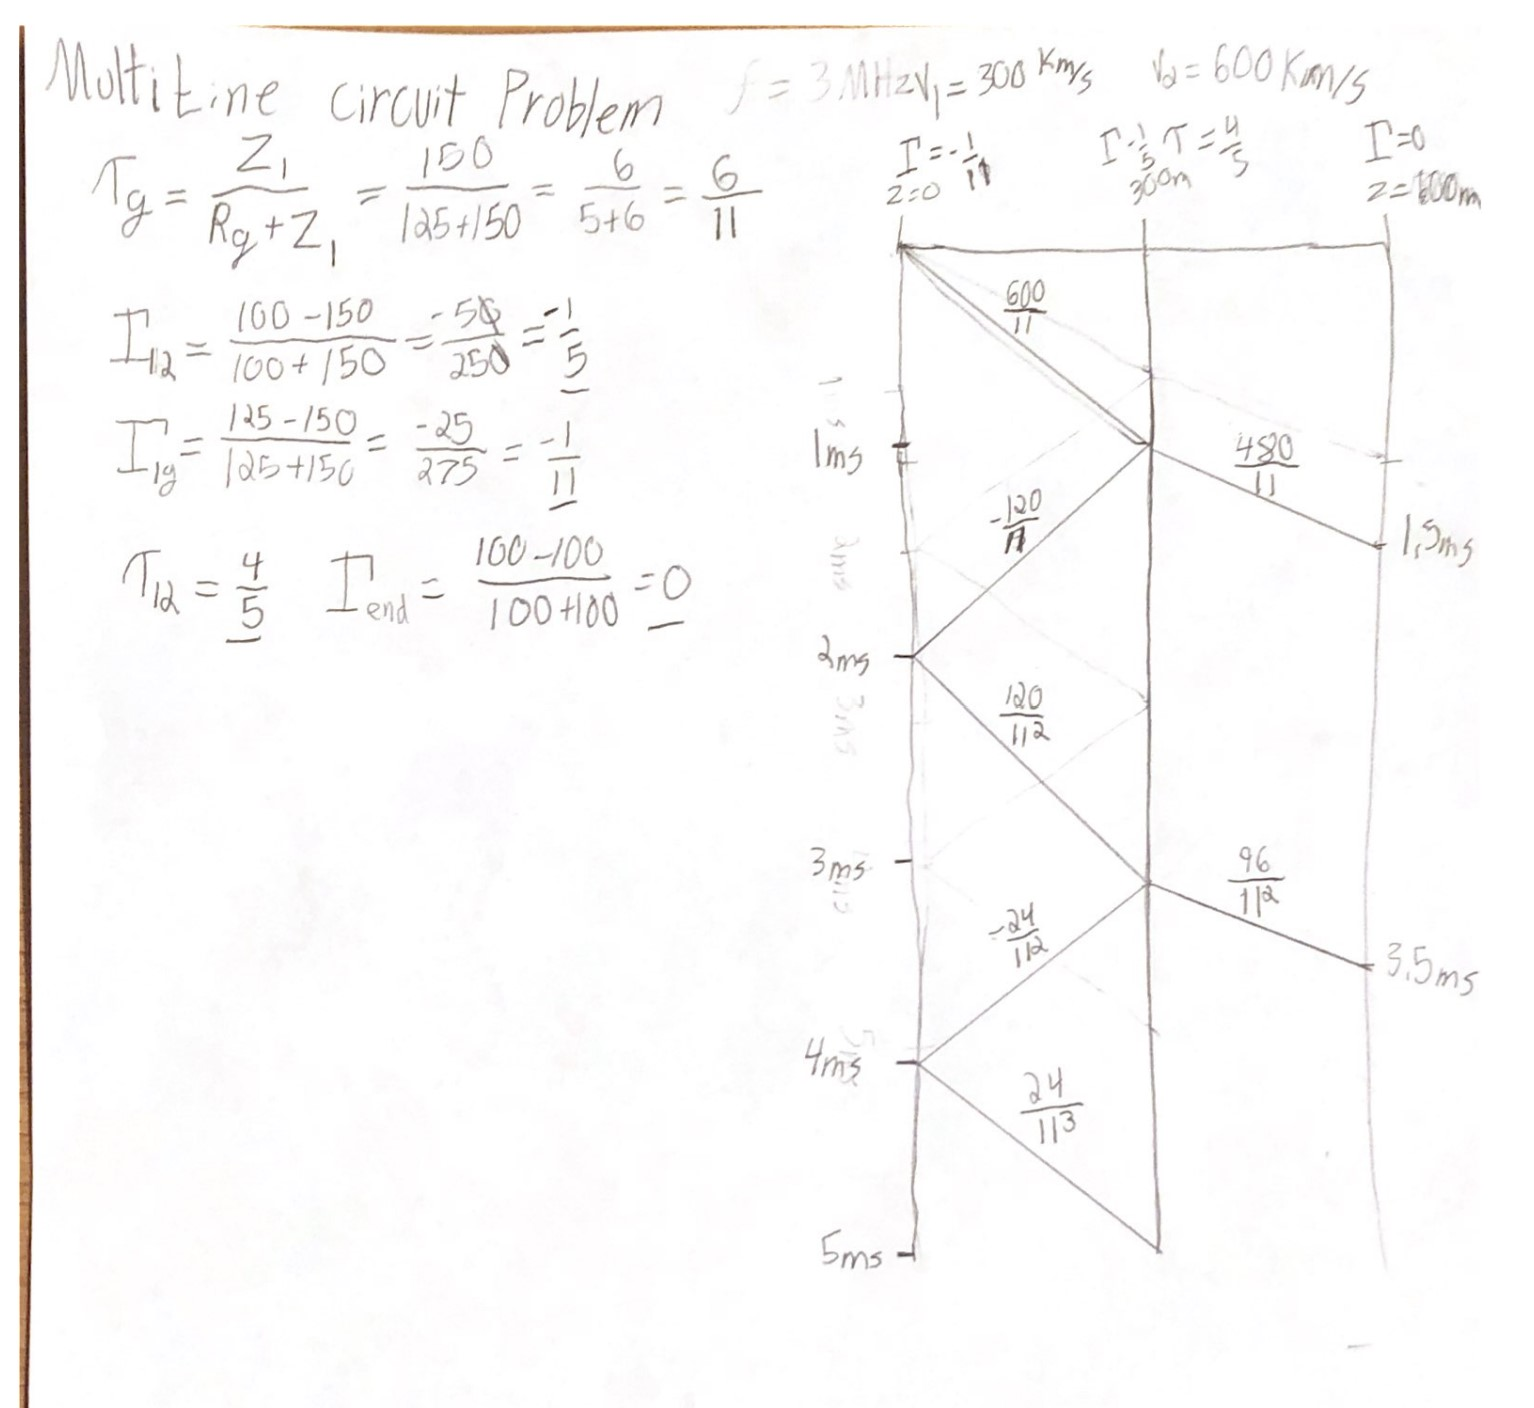
\includegraphics[width=
    \textwidth]{figures/Multiline_Solution.jpg}
\end{center}
\end{figure}

\newpage

\section{Terrific Transforms}

\begin{figure}[H]
\begin{center}
    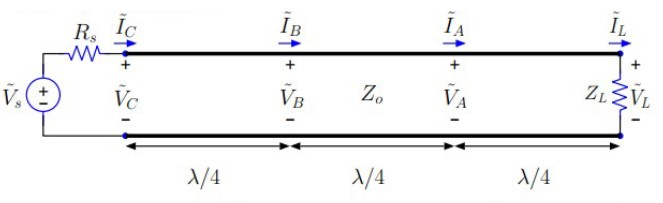
\includegraphics[width=0.93\textwidth]{figures/329 Problem 2.jpg}
\end{center}
\end{figure}

In the circuit above, $Z_0 = 50 \Omega$, $Z_L = 25 + j25 \Omega$, $R_s = 50 \Omega$, and $\tilde{V}_s = 20 V$. The line length if $3 \lambda / 4$. Answer the following questions:

\subsection{Solution:}

\begin{enumerate}
    \item \textbf{Determine impedance $\tilde{V}_B/\tilde{I}_B$ and explain.}

    At point $B$ we are $\lambda/2$ away from the load. This is a full rotation on the Smith Chart, so we can simply copy the load impedance. $\boxed{25 + j25 \Omega}$

    \vfill
    
    \item \textbf{Determine impedance $\tilde{V}_C/\tilde{I}_C$ and explain.}

    Recall the quarter-wave transformer for impedances:

    $$Z_{in} = \frac{Z_0^2}{Z_L}$$

    Point $C$ is a quarter-wavelength away from point $B$, so we can plug it in and simplify.

    $$Z_{in} = \frac{50^2}{25 + j25} = \frac{100}{1 + j} = \frac{100(1 - j)}{(1 + j)(1 - j)} = \frac{100 - j100}{1 + 1}$$

    $$= \boxed{50 - j50 \Omega}$$

    \vfill
    
    \item \textbf{Use voltage division to determine voltage $\tilde{V}_C$ and show work.}

    We calculated the input impedance in the previous part, so now we can just perform voltage division to get $\tilde{V}_C$.

    $$\tilde{V}_C = 20 \left(\frac{50 - j50}{50 - j50 + 50} \right) = 20 \left(\frac{1 - j}{2 - j} \right) = 20 \left(\frac{(1 - j)(2 + j)}{(2 - j)(2 + j)} \right) = 20 \left(\frac{3 - j}{5} \right)$$

    $$= \boxed{12 - j4 V}$$

    \vfill
    \newpage
    
    \item \textbf{Determine $\tilde{V}_A$ and explain.}

    Point $A$ is half a wavelength away from point $C$, so we simply multiple $\tilde{V}_C$ by $-1$ to get $\tilde{V}_A$. $\boxed{-12 + j4 V}$

    \vfill
    
    \item Determine $\tilde{I}_L$ using the ``current forcing formula'' from $\tilde{V}_A$.

    Recall that the current forcing formula works when we want to find the current a quarter-wavelength towards the source from a position where we know the voltage. We use it here, taking the answer from the previous part.

    $$\tilde{I}_L = -j \frac{\tilde{V}_A}{Z_0} = -j \left(\frac{-12 + j4}{50}\right)$$

    $$= \boxed{\frac{2}{25} + j\frac{6}{25} A}$$

    \vfill
    
    \item \textbf{Determine the average power absorbed in $Z_L$.}

    Recall that for phasors we find the average power a bit differently. But first, we need to find $\tilde{V}_L$.

    $$\tilde{V}_L = \tilde{I}_L Z_L = \left(\frac{2}{25} + j\frac{6}{25}\right)\left(25 + j25 \right) = 2 + j6 + j2 - 6 = -4 + j8 V$$

    Now we find average power.

    $$P_L = \frac{1}{2} \text{Re}\{\tilde{V}_L \tilde{I}_L^*\} = \frac{1}{2} \text{Re}\{(-4 + j8) \left(\frac{2}{25} - j\frac{6}{25}\right)\} = \frac{1}{2} \text{Re}\{\frac{-8}{25} + j\frac{16}{25} + j\frac{24}{25} + \frac{48}{25}\} = \frac{1}{2} \frac{40}{25}$$

    $$= \boxed{0.8 W}$$

    \vfill
    
    \item \textbf{Determine $\tilde{I}_B$ and explain.}

    Point $B$ is a half-wavelength away from the load. The current simply changes sign when we move half a wavelength along the line. THerefore, $\tilde{I}_B = -\tilde{I}_L = \boxed{-\frac{2}{25} - j\frac{6}{25} A}$

    \vfill
    \newpage
    
\end{enumerate}

\newpage

\section{Sly Smith Charts}
\label{section:smith_chart}

The following is a series of conceptual questions meant to poke and prod at your understanding of Smith Charts.

\subsection{Magnificent Motivation}

Why do we use Smith Charts? What's wrong with our easy quarter-wave and half-wave transformers?

\textcolor{red}{It turns out that transmission lines might not have lengths equal to a quarter-wavelength or a half-wavelength. So we need to do some nasty math instead.}

\vfill

\subsection{Formal Formulae}
\label{section:formal_formulae}

Consider a TL with intrinsic impedance $Z_0$ and arbitrary length $l$ terminated by an arbitrary load $Z_L = R_L + jX_L$.

What is the equation for the voltage and current on the line at some arbitrary distance $d$ from the load in terms of the forward-going voltage $V^+$, the backward-going voltage $V^-$, the wave number $\beta$, and the intrinsic impedance of the TL $Z_0$?

\textcolor{red}{$V(d) = V^+ e^{j\beta d} + V^- e^{-j \beta d}$}

\textcolor{red}{$I(d) = \frac{V^+ e^{j\beta d} - V^- e^{-j \beta d}}{Z_0}$}

\vfill

\subsection{Realistic Reflections}
\label{section:realistic_reflections}

Now let us define the load reflection coefficient to be $\Gamma_L = \frac{Z_L - Z_0}{Z_L + Z_0}$. This should look familiar - it has a very similar form to the reflection coefficients from waves hitting a boundary!

Rewrite your answers from Section \ref{section:formal_formulae} in terms of $V^+$, $\Gamma_L$, $\beta$ and $Z_0$.

\textcolor{red}{$V(d) = V^+ e^{j\beta d}(1 + \Gamma_L e^{-j2 \beta d})$}

\textcolor{red}{$I(d) = \frac{V^+ e^{j\beta d}(1 - \Gamma_L e^{-j2\beta d})}{Z_0}$}

\vfill

\subsection{Redefining Reflections}
\label{section:redefining_reflections}

Let's define a generalized reflection coefficient to be $\Gamma(d) = \Gamma_L e^{-j2 \beta d}$.

Rewrite your answers in Section \ref{section:realistic_reflections} in terms of $V^+$, $\Gamma(d)$, $\beta$, and $Z_0$. Also explain the significance of $\Gamma(d)$ - what does it mean when someone says $\Gamma(3) = 0.5$? What ranges of values can $\Gamma(d)$ take?

One important property of $\Gamma(d)$ is that it has a constant magnitude $\Gamma_L$ for all $d$ - only the phase changes. How is this represented on the Smith Chart?

\textcolor{red}{$V(d) = V^+ e^{j\beta d}(1 + \Gamma(d))$}

\textcolor{red}{$I(d) = \frac{V^+ e^{j\beta d}(1 - \Gamma(d))}{Z_0}$}

\textcolor{red}{When someone says $\Gamma(3) = 0.5$, they mean that if we were to replace the load and the transmission line of length three units with just a lumped circuit load that caused $\Gamma_L = 0.5$, we would see no difference in what is reflected back towards the generator and the standing wave that is formed in steady state conditions.}

\textcolor{red}{$\Gamma(d)$ can take on any value on or within the unit circle on the complex plane - recall that $\Gamma_L$ can only take on values between -1 and 1.}

\textcolor{red}{On the Smith Chart this is represented as the giant circle and all the concentric circles that you draw on the Smith Chart with your compass! The giant circle has a radius of 1, signifying that it is indeed a unit circle.}

\vfill
\newpage

\subsection{Intuitive Impedance}

Impedance, as a concept, is usually seen as voltage over current. Thus, take the equation for $V(d)$ that you found in \ref{section:redefining_reflections} and divide it by the equation for $I(d)$. Let's call this $Z(d)$. What is $Z(d)$?

\textcolor{red}{$Z(d) = Z_0 \frac{1 + \Gamma(d)}{1 - \Gamma(d)}$}

\vfill

\subsection{Quality Question}

A fellow student protests - "I thought the ratio between the voltage and current on the transmission line was always the intrinsic impedance of the transmission line, namely $Z_0$!"

Is the student wrong? Justify your answer.

\textcolor{red}{That ratio is correct only in VERY special scenarios when $\Gamma_L$ isn't complex, and also only in the "DC" case where we work in the TIME domain with delta inputs. However, this statement is already untrue in the DC case - if you put a unit-step input onto a transmission line, you end up with superposed forward and backward going waves, which will not follow this ratio either. And we're not even in the time domain anymore - everything we work with is in the phasor domain.}

\textcolor{red}{Bounce diagrams use this ratio because they deal with delta inputs. And if you examine the forward and backward going waves individually, you will find that the ratio of voltage to current is indeed still $Z_0$. However we no longer want to watch transient responses on a transmission line - we're going for the steady state solution instead. Thus we don't care about individual $V^+$ and $V^-$ anymore - instead we care about the superposition of all $V^+$s and $V^-$s. And therefore we lose that nice relationship between voltage and current for now. So nothing actually changed! We just added a layer of abstraction.}

\vfill

\subsection{Noble Normalizations}

We find it convenient to normalize $Z(d)$, since we would like to generalize our example to transmission lines of any $Z_0$, not just a specific $Z_0$. Therefore, we define $z(d) = \frac{Z(d)}{Z_0}$.

We would also like to rewrite $\Gamma(d)$ in terms of $Z(d)$ and $Z_0$, for reasons we'll see later.

We also are going to stop writing $(d)$ everywhere because it is clear that these are functions of $d$.

Find $z(d)$ in terms of $\Gamma$ and find $\Gamma$ in terms of $Z$ and $Z_0$.

\textcolor{red}{$z(d) = \frac{1 + \Gamma}{1 - \Gamma}$}

\textcolor{red}{$\Gamma = \frac{Z - Z_0}{Z + Z_0}$}

\vfill

\subsection{Interesting Intermission}

This nice-looking relationship between $\Gamma$ and $z$ is known as a bilinear transformation, where bilinear refers to the fact that the numerator as well as the denominator of these transformations are linear with respect to the variable being transformed.

If you've taken ECE310 or are in it right now, then this is not the first bilinear transformation you've seen. The Laplace Transform and the z-transform also have a bilinear transformation between them, namely

$$H(z) = H_L(s) \vert_{s = \alpha \frac{1 - z^{-1}}{1+z^{-1}}}$$

Indeed, these two transformations are closely linked - their stability and causality conditions all map from one domain to the other flawlessly. And yes, the general shape of the transformation looks very similar to the Smith Chart.

More details of this can be found in MATH446 - Applied Complex Variables. But alas, I digress. Back to Smith Charts.

\newpage

\subsection{Synthetic Shapes}

What are the lines on the Smith Chart that denote constant $r$ and constant $x$, where $z = r + jx$? Why do they look so weird and all over the place?

We define the normalized line admittance to be $y(d) = y = \frac{1}{z}$. Given a $z$ on the Smith Chart, where is $y$? Why?

\textcolor{red}{Constant $r$ are the big circles whose centers slide further and further to the right as the radius of each circle gets smaller.}

\textcolor{red}{Constant $x$ are the weird curved lines that seem to emanate from the right-hand point of the Smith Chart and bloom over the entire chart.}

\textcolor{red}{Given a $z(d)$, the $y(d)$ is located opposite the origin from $z(d)$. Usually one finds this by drawing a circle centered at the origin that passes through $z(d)$, and then placing a ruler from $z(d)$ through the origin and using the other point on the circle that $z(d)$ crosses.}

\textcolor{red}{Verification: $y = \frac{1}{z} = \frac{1 - \Gamma}{1 + \Gamma} = \frac{1 + (-\Gamma)}{1 - (-\Gamma)}$. Since we know that $z$ is the transform of $\Gamma$, $y$ must be the transform of $-\Gamma$. Adding a minus sign on $\Gamma$ indeed means going to the opposite side of the constant $\Gamma$ circle (we add a phase of 180 degrees to invert a phasor).}

\vfill

\subsection{Pivotal Points}

What does the origin of the Smith Chart correspond to in terms of $\Gamma$? What does the origin of the Smith Chart correspond to in terms of $z$? What does the origin of the Smith Chart correspond to in real life?

What does the leftmost point of the Smith Chart correspond to in terms of $\Gamma$? What does the leftmost point of the Smith Chart correspond to in terms of $z$? What does the leftmost point of the Smith Chart correspond to in real life?

What does the rightmost point of the Smith Chart correspond to in terms of $\Gamma$? What does the rightmost point of the Smith Chart correspond to in terms of $z$? What does the rightmost point of the Smith Chart correspond to in real life?

\textcolor{red}{At the origin $\Gamma(d) = \Gamma_L = 0$, since phase is irrelevant. $z = 1 + 0j$. This corresponds to the case where we have a matched load - there is no reflection, and $z(d)Z_0 = Z_0$ no matter how we rotate ourselves.}

\textcolor{red}{At the leftmost point $\Gamma(d) = -1$. $z = 0 + 0j$. Recall what it means when $z(d)Z_0 = 0$ - this means there is no voltage, so we have an short circuit. If this location is where our load is, then our load is a short circuit $(z(0)Z_0 = 0$, aka there is no impedance at the load!)}

\textcolor{red}{At the rightmost point $\Gamma(d) = 1$. $z = \infty$. Recall what it means when $z(d)Z_0 = \infty$ - this means there is no current, so we have a open circuit. If this location is where our load is, then our load is an open circuit $(z(0)Z_0 = \infty$, aka there is infinite impedance at the load!)}

\vfill
\newpage

\subsection{Devious Details}

Let's now go over some of the methods that you've probably used when dealing with Smith Charts. We'll see if you know why those methods actually work.

\begin{enumerate}
    \item Matthew tells you that at the load end of the transmission line he's at angle 0 on the Smith Chart. He then walks 3 meters toward the input and asks what angle we're at now. What information are you missing to solve this problem? Why is it important?
    \item Matthew restarts at the load and walks $\frac{\lambda}{2}$ distance towards the input. How many degrees did he walk through on the Smith Chart? Why?
    \item Matthew receives a transmission line problem with some load impedance and some intrinsic impedance. He first normalizes the load impedance, enters it on the Smith Chart, and then draws a constant gamma circle that passes through the origin and the point he drew. Why did he do each of these three steps?
    \item Matthew finds the input impedance of some transmission line setup. He enters it on the Smith Chart and finds the phase and magnitude of $\Gamma$ at that point. What is the significance of this $\Gamma$?
    \item When travelling towards the source Matthew always rotates clockwise along the Smith Chart. Why? If Matthew instead travels towards the load then which direction should he rotate?
    \item Does the Smith Chart give you steady state solutions, transient solutions, or both?
\end{enumerate}

\textcolor{red}{
\begin{enumerate}
    \item He didn't tell us the wavelength. The length of a transmission line with respect to the wavelength of the wave propagating down the line is what is important (and thus is often referred to as electrical length). Without this information we have no idea how long the transmission line is with respect to the wavelength so we don't know what phase we're at, etc.
    \item He walks a full 360 degrees counterclockwise around the Smith Chart. Recall that $\Gamma(d) = \Gamma_L e^{-j2\beta d}$. Substituting $\beta = \frac{2 \pi}{\lambda}$ and $d = \frac{\lambda}{2}$, we get that $\Gamma(\frac{\lambda}{2}) = \Gamma_L e^{-j2 \pi} = \Gamma_L$. A distance of $\frac{\lambda}{2}$ will always take us right back where we started because of the 2 in $\Gamma(d)$'s equation.
    \item He normalizes the load impedance because the Smith Chart deals with normalized load impedances only (this is so it can work for all transmission line intrinsic impedances). He enters it on the Smith Chart because why not (like literally, there's no reason not to unless you're not going to use a Smith Chart). He draws a constant $\Gamma$ circle that passes through that point because the Smith Chart provides the bilinear transform for us. By drawing the circle, he essentially found what $\Gamma_L$ is. Since $\Gamma$'s magnitude never changes, he is now free to draw a constant $\Gamma$ circle that represents the fact that the magnitude never changes.
    \item If he were to collapse the entire transmission line and the load into a single resistor such that $\Gamma$ remained the same as the $\Gamma$ he found, the generator wouldn't know the difference. Recall that we're in steady state.
    \item Recall that $\Gamma(d) = \Gamma_L e^{-j2\beta d}$. This means that the phase decreases (or goes clockwise) as $d$ increases. This is why we rotate clockwise. If he were to travel towards the load, then $d$ would be decreasing, so he would need to travel counterclockwise.
    \item Steady state only!!! There are no transient responses here, which is why all we see on the transmission line is a standing wave (no galloping, just a cosinusoidal variation with respect to time at with magnitude determined by the standing wave at each specific point on the line). To find the transient solution we would either have to do some bounce diagram stuff (disgusting) or return to Laplace Transforms (slightly better, still not fun).
\end{enumerate}}

\section{Quintessential Quarter-Wave}

A quarter-wave transformer will be inserted on the transmission line shown below some distance $d$ away from the load. Find $d$ and the optimal intrinsic impedance of the line to be inserted $Z_q$ such that the load depicted is a perfect match.

\begin{figure}[h]
\begin{center}
    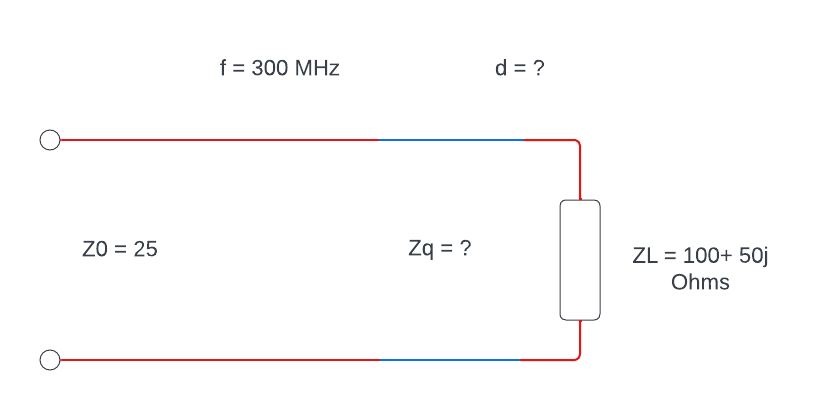
\includegraphics[width= 0.8
    \textwidth]{figures/Quarter_wave_transformer.png}
\end{center}
\end{figure}

Assume that $f = 300$MHz. Use a Smith Chart if you think you need one. Recall what you learned in Section \ref{section:smith_chart} and try and justify every step that you make.

\begin{figure}[H]
\begin{center}
    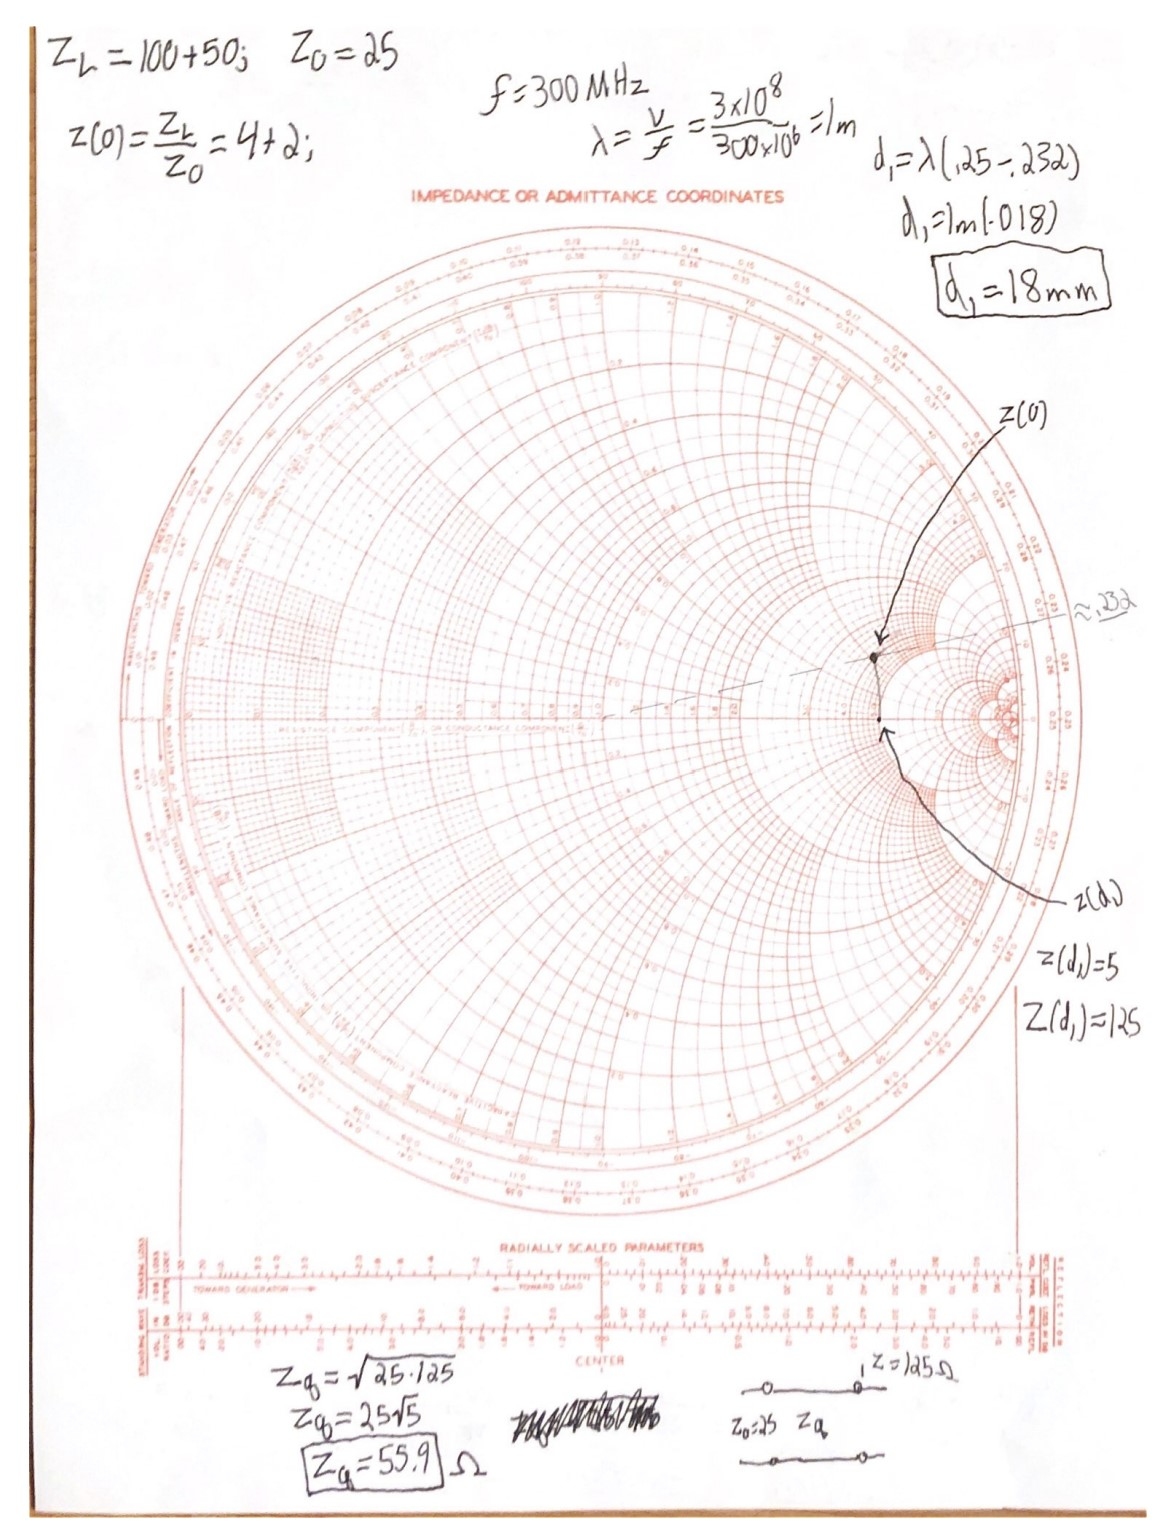
\includegraphics[width= 0.8
    \textwidth]{figures/Quarter_transformer_solution.jpg}
\end{center}
\end{figure}

\newpage

\section{Vital VSWR}

Now that you have mastered Smith Charts, it's time to tackle the other difficult concept on the final - Voltage Standing Wave Ratio, or VSWR. Let's begin.

\subsection{Sedentary Standing Waves}

Here's a warmup question to get started - what is a standing wave?

\textcolor{red}{A standing wave is a vibration of a system  that does not propagate power in some direction (or in this case, propagates power less efficiently). There are locations of maximum maximum amplitude and minimum maximum amplitude (see the next section to figure out what this means).}

\vfill

\subsection{Monarchical Maxes and Mins}

Recall that $V(d) = V^+ e^{j \beta d} (1 + \Gamma_L e^{-j2\beta d})$ for any point on the transmission line that is a distance $d$ from the load, found earlier (if you do not remember why, go back and review! This is super important!)

What is the biggest value in magnitude that $V(d)$ can achieve? At what value of $d$ does this value appear? Note that we call this value of $d$ as $d_{max}$.

What is the smallest value in magnitude that $V(d)$ can achieve? At what value of $d$ does this value appear? Note that we call this value of $d$ as $d_{min}$.

For this problem assume that $\Gamma_L$ is a positive real number between and including 0 and 1.

\textcolor{red}{For the max value of $V(d)$, we want $\Gamma(d) = \Gamma_L e^{-j2\beta d}$ to be maximum. Then $\vert V(d) \vert_{max} = \vert V^+ \vert (1 + \vert \Gamma_L \vert)$. Since we know that $\Gamma_L$ is real, we therefore want $d$ to be a multiple of $\frac{\lambda}{2}$ so that the second exponential's phase is a multiple of $2 \pi$. Note that the first exponential's phase doesn't matter, since it simply adds a phase angle to the entire expression and we only want the magnitude of the whole expression.}

\textcolor{red}{For the minimum value of $V(d)$, we want $\Gamma(d) = \Gamma_L e^{-j2\beta d}$ to be minimum. Then $\vert V(d) \vert_{max} = \vert V^+ \vert (1 - \vert \Gamma_L \vert)$. Since we know that $\Gamma_L$ is real, we therefore want $d$ to be an odd multiple of $\frac{\lambda}{4}$ so that the second exponential's phase is an odd multiple of $\pi$. Note that the first exponential's phase doesn't matter, since it simply adds a phase angle to the entire expression and we only want the magnitude of the whole expression.}

\vfill
\newpage

\subsection{General Graphs}

Here is a graph that you may have seen before concerning $\vert V(d_{max}) \vert$ and $\vert V(d_{min}) \vert$. What is actually going on in the real world (in the time domain)?

\begin{figure}[h]
\begin{center}
    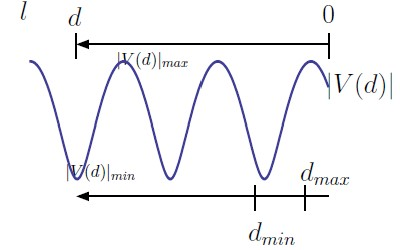
\includegraphics[width= 0.5
    \textwidth]{figures/Standing Wave Ratio.jpg}
\end{center}
\end{figure}

Hint: We have been almost exclusively dealing with what for half a semester?

Followup question: Does $z(d)$ or $\Gamma(d)$ depend on time? Why or why not?

\textcolor{red}{We have been dealing with phasors almost exclusively for the back half of the semester. As such, we must remember that the above image is not a time-domain plot, but a phasor-domain plot. Let's zoom in on one specific point in the line, say $d_{max}$. If we reintroduce time, then the voltage at this location will actually vary between $\vert V(d)_{max} \vert$, 0, go negative, hit 0 again, and then come back up. This is because when we convert a phasor to the time domain we will introduce a $cos(\omega t + \alpha)$ term, where $\alpha$ is some phase that is irrelevant to this conversation. Every single point on the line will also oscillate with respect to time in a similar fashion, only the amplitude will be dependent on what part of the line we're at.}

\textcolor{red}{Neither $z(d)$ or $\Gamma(d)$ depend on time. Voltage and current both have the same frequency, so any conversion on voltage to the time domain will also have a similar conversion on current, causing this conversion to cancel out when their ratio is taken. Don't believe me? Good. Take the voltage and current of some transmission line in steady state and divide voltage over current. You will find that the result has no dependence on time. Since $z$ and $\Gamma$ are related through a bilinear transform, if $z$ has no dependence on time then $\Gamma$ doesn't either.}

\vfill

\subsection{Clever Convenience}

We want a standing wave ratio, so it seems logical that we should divide the maximum magnitude of $V(d)$ with the minimum magnitude of $V(d)$. Perform this calculation. Does the result seem familiar?
 
\textcolor{red}{$VSWR = \frac{1 + \vert \Gamma_L \vert}{1 - \vert \Gamma_L \vert}$}

\vfill

\subsection{Interesting Intermission 2}

Let's do a quick comparison.

$$VSWR = \frac{1 + \vert \Gamma_L \vert}{1 - \vert \Gamma_L \vert} \text{ and } \vert \Gamma_L \vert = \frac{VSWR - 1}{VSWR + 1}$$

$$z = \frac{1 + \Gamma}{1 - \Gamma} \text{ and } \Gamma = \frac{z - 1}{z + 1}$$

Yup. It's another bilinear transformation.

We note now that $\Gamma(d_{max}) = \vert \Gamma_L \vert$ (hopefully you saw this from the earlier parts). Therefore,

$$VSWR = \frac{1 + \vert \Gamma_L \vert}{1 - \vert \Gamma_L \vert} = \frac{1 + \Gamma(d_{max})}{1 - \Gamma(d_{max})}$$

So where is VSWR on the Smith Chart, and why is it where you specified?

\textcolor{red}{Recall that at $d = d_{max}$, $\Gamma(d) = \vert \Gamma_L \vert$ since we're maximizing the possible voltage at that point on the line. We know that $\Gamma = \frac{z-1}{z+1}$, which means that at $d = d_{max}$, $VSWR = z(d_{max})$!}

\textcolor{red}{Since $\Gamma(d_{max}) = \vert \Gamma_L \vert$ and we know that $\vert \Gamma_L \vert$ is the rightmost point on the constant $\Gamma$ circle (where else could $\Gamma(d) = \vert \Gamma_L \vert$?), we know that VSWR is then the $z$ value corresponding to the rightmost point on the constant $\Gamma$ circle. That's pretty cool - knowing VSWR, aka a single number, will tell us a lot about the transmission line. VSWR also happens to be quite easy to find in the lab.}

\vfill

\subsection{Electric Extremes}

What are the extreme values that VSWR can take on? What situations do they represent in real life?

\textcolor{red}{If VSWR = 1, then $\Gamma(d) = \Gamma_L = 0$. This makes sense - if $\Gamma_L = 0$, then there is no reflection, so no standing wave will develop.}

\textcolor{red}{If VSWR = $\infty$, then $\vert \Gamma_L \vert = 1$. This makes sense - if $\vert \Gamma_L \vert = 1$, then we must have a short, open, or purely reactive load that is causing a perfect reflection. All of these cases correspond to the possibility of have $V = 0$ somewhere on the line, which would cause VSWR to blow up to $\infty$.}

\vfill
\newpage

\section{Short and Stubby}

A transmission line with an intrinsic impedance of 300 $\Omega$ is connected to a load impedance of $450-j600$ and a signal with frequency $10$MHz. Find the position and length of a short-circuited stub required to match the line using a Smith Chart.

Don't just blindly apply the method you learned in class - instead think about why each step makes sense as you do it. There's no guarantee that the final exam will only contain simple impedance matching like what you learned in class.

\subsection{Solution:}

Let's go through each step, one at a time. We do need the wavelength first. We're given that $f = 10$MHz, so $\lambda = c/f$ implies that $\lambda = 30$m. Now we can proceed.

\begin{enumerate}
    \item First we normalize the load impedance and plot it on the Smith Chart. We have to normalize, because the Smith Chart deals with normalized impedances in order to remain general.

    $$z_L = \frac{Z_L}{Z_0} = \frac{450 - j600}{300} = 1.5 - j2$$

    This is plotted at point A in the Smith Chart.

    \item We now convert this to a normalized admittance and plot it on the Smith Chart. This is useful because we're trying to attach a stub in parallel. Admittances simply add when combining things in parallel, hence why they are so useful.

    $$y_L = \frac{1}{z_L} = 0.24 + j0.32$$

    This can also be done graphically on the Smith Chart by drawing the constant gamma circle that intersects $z_L$, then rotating by 180 degrees. This admittance is graphed as point B.

    \item Find the intersection between the constant gamma circle and the $r = 1$ circle. There are two points where this happens, marked C and D on the Smith Chart. Both are valid. We'll choose to go with point C because why not.

    Note that we use the $r = 1$ circle because, if we somehow were able to get rid of the imaginary component, we'd be left with $y = z = 1$, which when we unnormalize, will give us our perfect matched load. We then note that we're using a shorted stub, which means for the stub we use the $\gamma = 1$ circle. The input impedance is always going to be completely imaginary wherever we are on this circle, which gives us our method to get rid of the imaginary component and keep only the real $y = z = r = 1$.

    \item We now know exactly where we should insert our shorted stub. Point B was at $0.052\lambda$ on the Smith Chart, while Point C was at $0.182 \lambda$ on the Smith Chart. Travelling towards the generator means moving clockwise, so the distance we need to travel is simply given by $0.182 \lambda - 0.052 \lambda = 0.13 \lambda = \boxed{3.9 m \text{ from the load for the positioning}}$.

    So let's recap. We found the admittance at the load, which was point B. The admittance here was $0.24 + j0.32$. We then moved 3.9 meters towards the generator. This lands us at point C. At this point in the line, our admittance is $1 + j1.7$. 

    \item So now our admittance is $1 + j1.7$. If we were to add an admittance $-j1.7$, we would only have a admittance of $1$, which is what we want for a matched load. So we find the point $0 - j1.7$ on the Smith Chart. This is marked as point E on the Smith Chart.

    A short has an admittance of infinity, so it starts on the right end of the Smith Chart. We then rotate clockwise towards the generator until we hit point E. This results in a $0.085\lambda$ movement, or a distance of $\boxed{2.55 m}$. This is the length of our shorted stub!
    
\end{enumerate}

\begin{figure}[H]
\begin{center}
    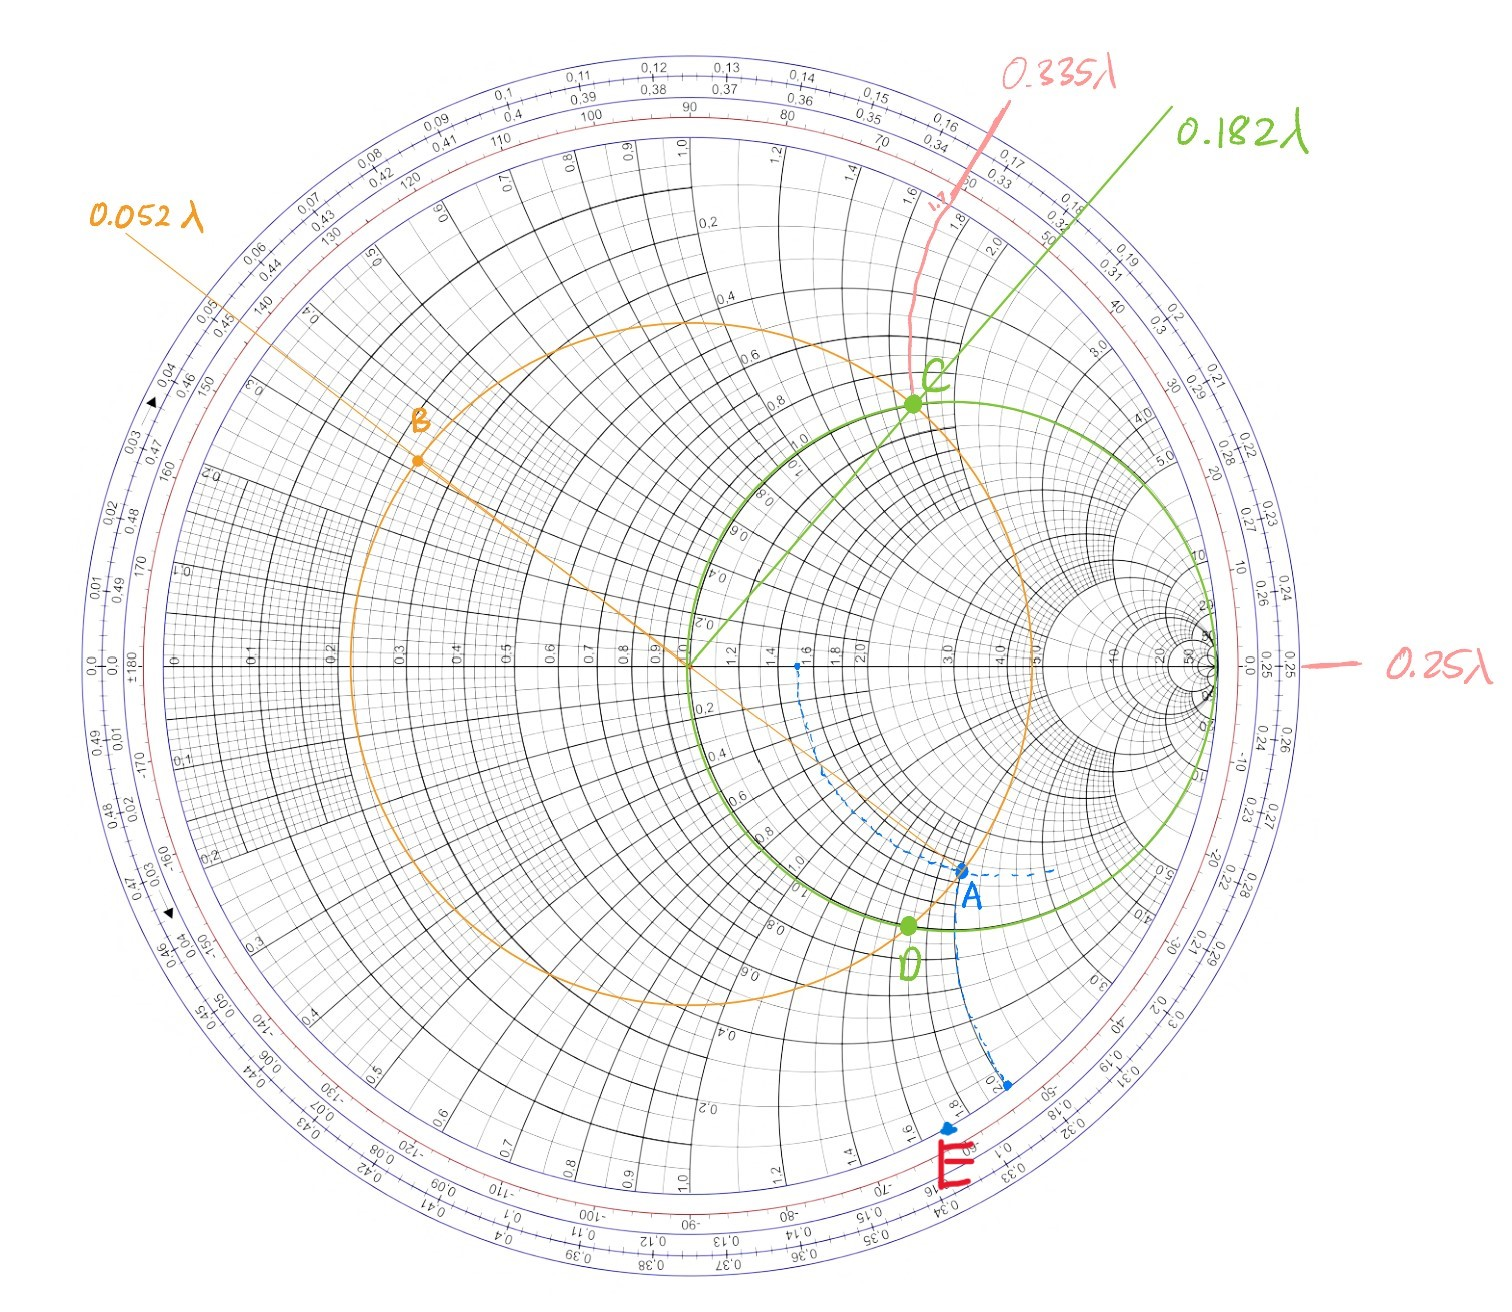
\includegraphics[width= 0.9
    \textwidth]{figures/Stubby Solution 2.jpg}
\end{center}
\end{figure}

\section{Rebellious Resonance}

A lossless transmission line of length 600 meters is left open at $z = 0$ and shorted at $z = l = 600$m. Determine the resonant frequencies of the line.

\subsection{Solution:}

We have a transmission line that's open at one end and shorted on the other. The resonant frequencies then must be the ones that make $600$ meters look like an odd multiple of $\lambda/4$. Recall that $\lambda = c/f$.

$$600 = (2n + 1) \lambda/4$$

$$600 = (2n + 1) \frac{c}{4f}$$

$$\boxed{f = \frac{1}{8} (2n + 1) MHz}$$

The above solution is valid for any $n \geq 0$.

\section{Daunting Distance}

\begin{figure}[H]
\begin{center}
    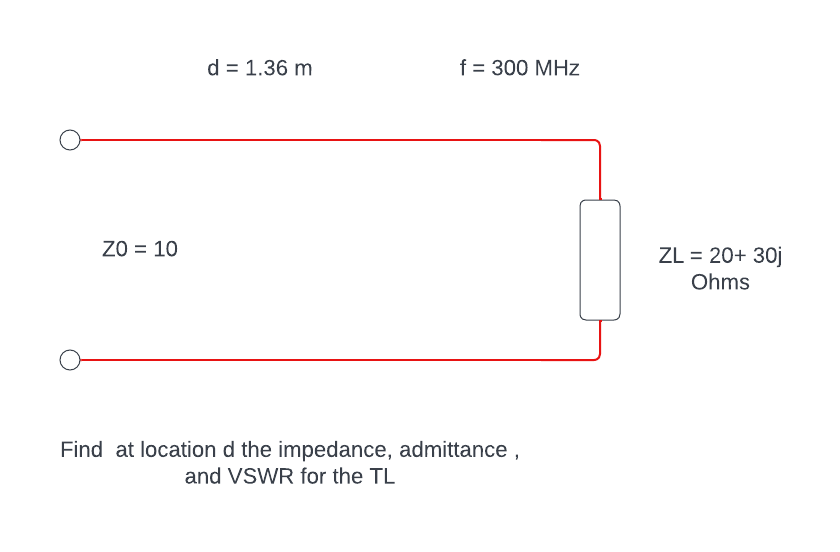
\includegraphics[width= 0.7
    \textwidth]{figures/VSWR Example.png}
\end{center}
\end{figure}

Assume that $f = 300$MHz. Also assume a velocity of $c$. Use a Smith Chart if you think you need one. Recall what you learned in Section \ref{section:smith_chart} and try and justify every step that you make.

\begin{figure}[H]
\begin{center}
    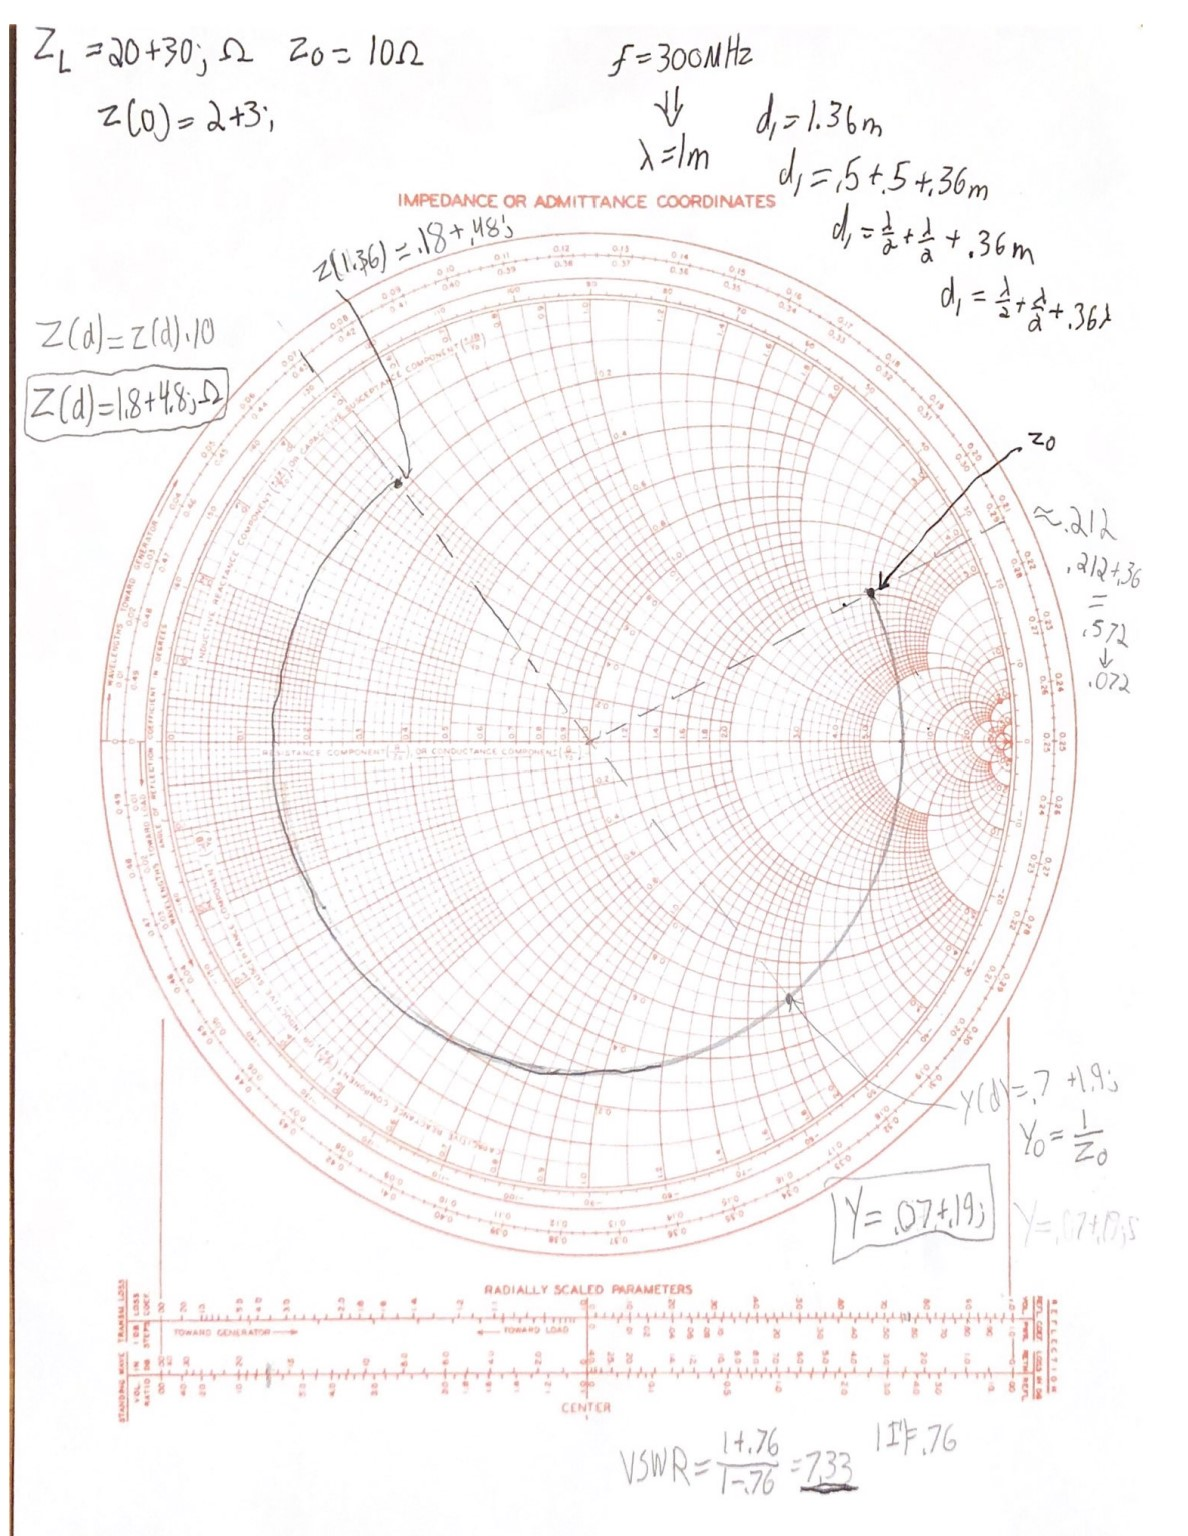
\includegraphics[width= 0.9
    \textwidth]{figures/Distance Solution.jpg}
\end{center}
\end{figure}

\textcolor{red}{Correction: $Y=0.07-0.19j$ -- the imaginary part is negative on the bottom half of the Smith Chart!}

\newpage

\section{Copious Coils}
A rectangular coil of dimensions a and b and resistance R moves with constant velocity v into a magnetic field as show below.

\begin{figure}[H]
\begin{center}
    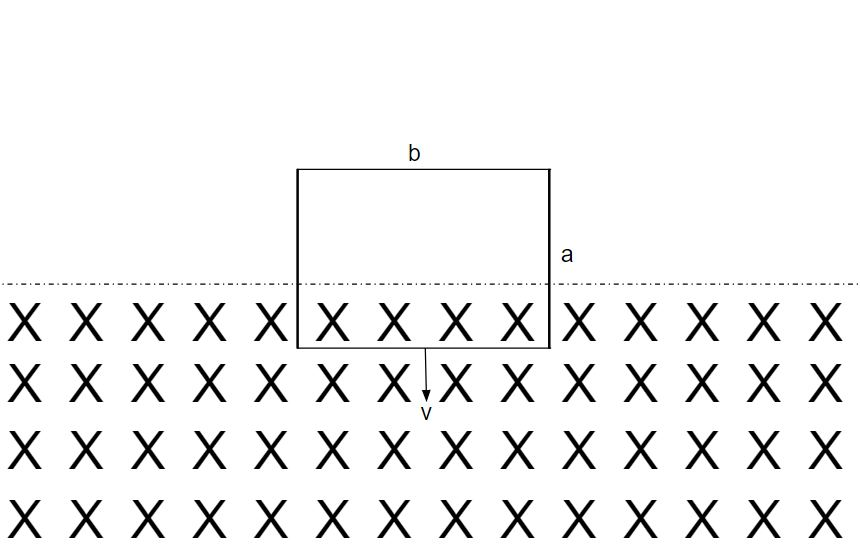
\includegraphics[width= 0.5\textwidth]{figures/square.jpg}
\end{center}
\end{figure}
\begin{enumerate}
    \item What is the emf induced in the coil? Express your answer in the appropriate units.
    \item What is the associated current? Express your answer in the appropriate units.
    \item What is the direction of the current flow?
\end{enumerate}
\subsection{Solution:} 
\begin{enumerate}
    \item Hilariously, the problem does not give a direction for coil. So there are two correct answers here. We give the one where the loop circulates clockwise (with normal vector pointing into the page in the direction of the B-field). We then arbitrarily assign the B-field direction to be $\hat{y}$, because we can.
    \begin{equation}
            \Phi = \int \int \Vec{B} \cdot d\Vec{S} = \int_{0}^{a} \int_{0}^{b} (B_0 \hat{y}) \cdot (\hat{y})=B_0 a(t)b \nonumber
          \end{equation}
          \begin{equation}
            a(t) = v_0 t\nonumber
          \end{equation}
          \begin{equation}
            \mathcal{E}=-\frac{d\Phi}{dt} = -B_0 b v_0 \nonumber
          \end{equation}
    \item Plug and chug.
    \begin{equation}
            \mathcal{E}=IR \nonumber
          \end{equation}
          \begin{equation}
            I=\frac{\mathcal{E}}{R} = -\frac{B_0 b v}{R}A \nonumber
          \end{equation}
    \item We chose our loop to be in the clockwise direction, and the current we found was negative. So the current is actually counterclockwise!
\end{enumerate}

\newpage

\section{Famous Fields}

In a homogenous medium, show that the phasor electric field in a source-free region satisfies the following relation, where $\beta$ is the wavenumber. DO NOT use your notes or textbook!

\[
\nabla^2 \tilde{E} + \beta^2\tilde{E} = 0
\]

Hint: $\nabla\times(\nabla\times \tilde{E}) = \nabla(\nabla \cdot \tilde{E}) - \nabla^2 \tilde{E}$.

\subsection{Solution:}

When in doubt, always return to Maxwell's equations. We'll start by writing them down (and paying a tribute to Maxwell).

$$\vec{\nabla} \cdot \vec{D} = \rho$$
$$\vec{\nabla} \cdot \vec{B} = 0$$
$$\vec{\nabla} \times \vec{E} = -\frac{\partial{\vec{B}}}{\partial t}$$
$$\vec{\nabla} \times \vec{H} = \vec{J} + \frac{\partial{\vec{D}}}{\partial t}$$

Let's convert these to phasor form first, since the problem asks for the phasor electric field.

$$\vec{\nabla} \cdot \tilde{D} = \tilde{\rho}$$
$$\vec{\nabla} \cdot \tilde{B} = 0$$
$$\vec{\nabla} \times \tilde{E} = -j \omega \tilde{B}$$
$$\vec{\nabla} \times \tilde{H} = \tilde{J} + j \omega\tilde{D}$$

Now we use one of the key pieces of information: we're in a source-free region! We now set $\tilde{\rho} = 0$ and $\tilde{J} = 0$.

$$\vec{\nabla} \cdot \tilde{D} = 0$$
$$\vec{\nabla} \cdot \tilde{B} = 0$$
$$\vec{\nabla} \times \tilde{E} = -j \omega \tilde{B}$$
$$\vec{\nabla} \times \tilde{H} = j \omega\tilde{D}$$

Oddly symmetric, huh? The hint seems to yell at us to take the curl of one of the bottom equations, so we happily oblige by taking the curl of one of them. We then set up the fourth equation, for funsies.

$$\vec{\nabla} \cdot \tilde{D} = 0$$
$$\vec{\nabla} \cdot \tilde{B} = 0$$
$$\vec{\nabla} \times (\vec{\nabla} \times \tilde{E}) = - j \omega (\vec{\nabla} \times \tilde{B})$$
$$\vec{\nabla} \times \mu \tilde{H} = j \mu \omega\tilde{D}$$

On the left side, we can then use the hint. On the right side, we can substitute the fourth equation into the third one. Since the medium is homogenous, $\mu$ can be safely pulled out of the curl without any damage.

$$\vec{\nabla} \cdot \tilde{D} = 0$$
$$\vec{\nabla} \cdot \tilde{B} = 0$$
$$\nabla(\nabla \cdot \tilde{E}) - \nabla^2 \tilde{E} = - j \omega (j \mu \omega\tilde{D})$$

The first equation can now be substituted in to destroy the first term on the left (gradient of $0$ is still $0$). We then drop the second equation - it is now useless.

$$- \nabla^2 \tilde{E} = \omega^2 \mu \epsilon \tilde{E}$$

Let's rearrange some equations. Recall also that in homogenous media, the propagation velocity through media is also given as $v^2 = \frac{1}{\mu \epsilon}$. We make this substitution.

$$\nabla^2 \tilde{E} - \frac{\omega^2}{v^2} \tilde{E} = 0$$

Recall the relation that defines the wave number: $\beta = \frac{\omega}{v}$. Thus,

$$\boxed{\nabla^2 \tilde{E} - \beta^2 \tilde{E} = 0}$$

\newpage

\section{Monumental Magnetics}

Consider an infinitely long conducting cylinder of radius $a$, with a cylindrical hole of radius $b$ placed at an offset $d$ from the center of the conductor. Assume that a static current $I$ is uniformly distributed across the cross-sectional area of the conductor. What is the magnitude of the magnetic field inside the hole?

\begin{figure}[H]
\begin{center}
    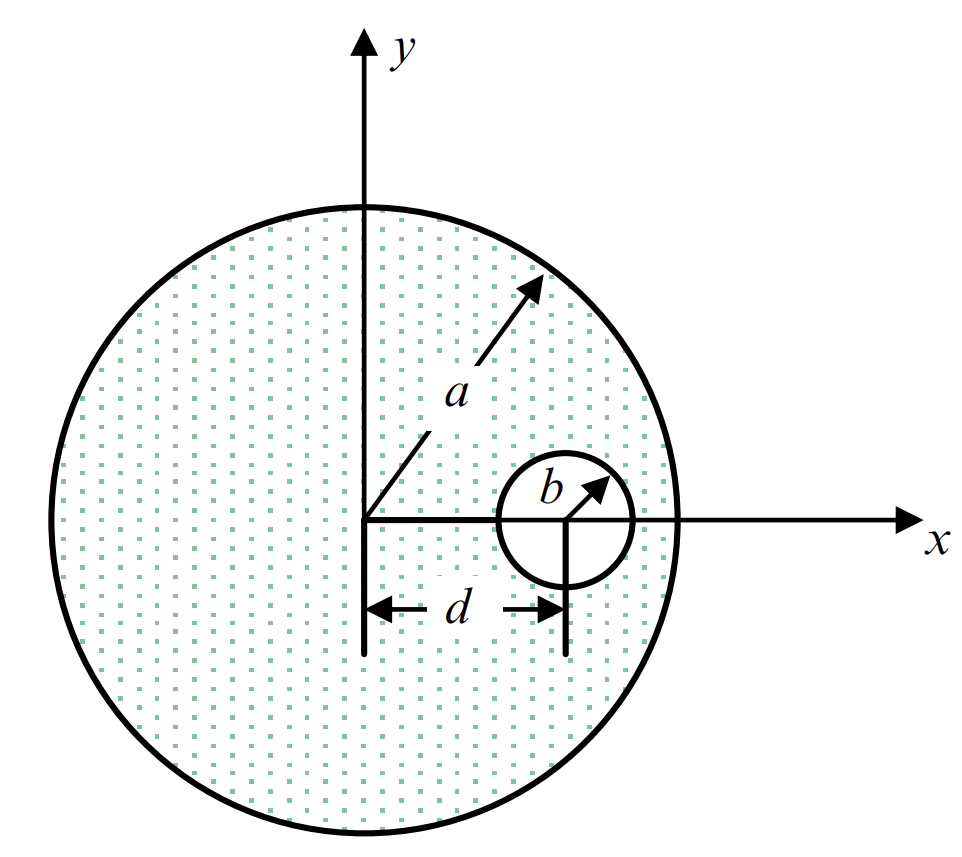
\includegraphics[width= 0.3\textwidth]{figures/cyl.png}
\end{center}
\end{figure}

\subsection{Solution:} This is a fairly standard problem in electromagnetics, with a somewhat surprising solution; the magnetic field inside the hole is $\textbf{uniform}$, with:

\[
B_{hole} = \frac{\mu_0 I d}{2\pi (a^2-b^2)}
\]

Consider a point P inside the hole, which is $\hat{s}_1$ away from the origin and $\hat{s}_2$ away from the center of the hole, which is a vector $\hat{d}$ away from the origin, i.e. $\hat{d} + \hat{s}_2 = \hat{s}_1$. 

\begin{figure}[ht!]
\centering
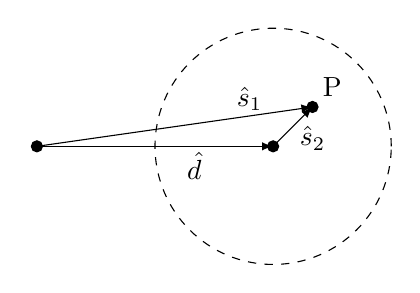
\begin{tikzpicture}

\node at (0,0) (A) {};
\node at  (3,0) (B) {};
\node at (3.5,0.5) (C) {};

\draw [-latex] (3,0) -- (3.5,0.5) {};
\draw [-latex] (0,0) -- (3,0) {};
\draw [-latex] (0,0) -- (3.5,0.5) {};
\draw [dashed] (B) circle (1.5);

\filldraw[black] (0,0) circle (2pt);
\filldraw[black] (3,0) circle (2pt);
\filldraw[black] (3.5,0.5) circle (2pt);

\node at (3.75,0.75) {P};
\node at (2,-0.25) {$\hat{d}$};
\node at (3.5,0.1) {$\hat{s}_2$};
\node at (2.7,0.6) {$\hat{s}_1$};


\end{tikzpicture}
\end{figure}

Now, we can consider the original problem as a superposition of two cylinders, both with a uniform current density $J$, with opposing signs, across each of them. Evidently, their superposition yields the original problem. 
\vspace{3mm}

At point $P$, we must then consider two magnetic field vectors, one from the larger cylinder and one from the smaller cylinder. 

\begin{figure*}[ht!]
    \centering
    \begin{subfigure}[b]{0.5\textwidth}
        \centering
        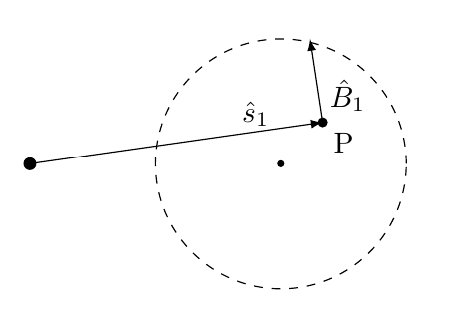
\includegraphics[width=0.5\linewidth]{figures/vec1.png}
        \caption{Field from Outer Cylinder}
    \end{subfigure}%
    ~ 
    \begin{subfigure}[b]{0.5\textwidth}
        \centering
        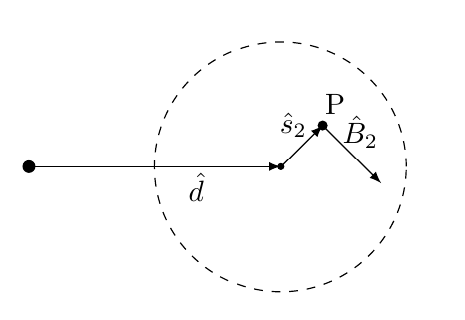
\includegraphics[width=0.5\linewidth]{figures/vec2.png}
        \caption{Field from Inner Cylinder}
    \end{subfigure}
    \caption{$\hat{B}_1$ and $\hat{B}_2$}
\end{figure*}

\newpage

 The B-field vector at point $P$ is then a superposition of fields $B_1$ and $B_2$, which are vectors obtained from Ampere's Law as follows:
\[
B\times 2\pi s = \mu_0 J \times \pi s^2 
\]

\[
\hat{B}_1 = \frac{\mu_0}{2} \hat{J}\times \hat{s}_1 \qquad \hat{B}_2 = -\frac{\mu_0}{2} \hat{J} \times \hat{s}_2
\]

Adding the two together leads to the conclusion that:

\[
\hat{B} = \frac{\mu_0}{2}\hat{J} \times(\hat{s}_1 - \hat{s}_2) = \frac{\mu_0}{2}\hat{J}\times\hat{d}
\]

Since $J$ in the expression above is the superposed current density, it is equal to $\frac{I}{\pi(a^2 - b^2)}$, we end up with the following result, also noting the orthogonality of $\hat{d}$ and $J$:

\[
B = \frac{\mu_0 I d}{2\pi (a^2 - b^2)}
\]
\newpage

\section{Deceptive Devices}

Consider the two devices below, with output and input impedances of 50 $\Omega$ and 200 $\Omega$ respectively. 

\begin{figure}[H]
\begin{center}
    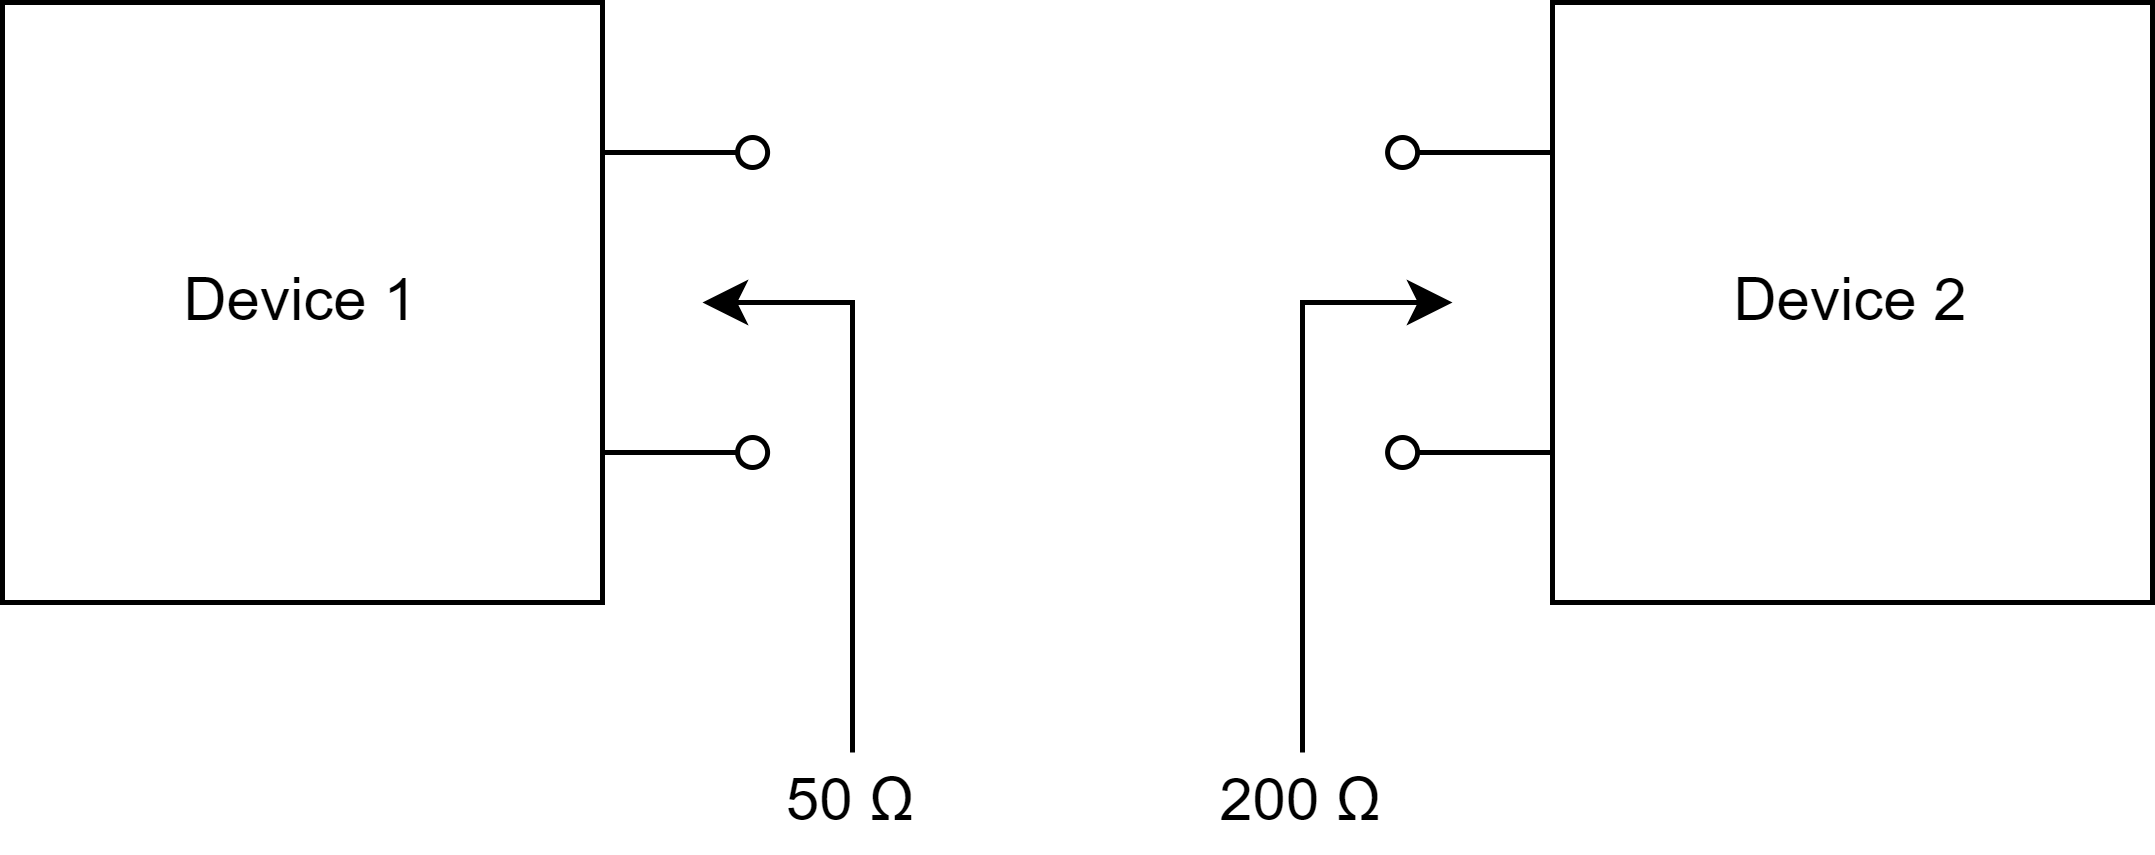
\includegraphics[width= 0.5\textwidth]{figures/matc.png}
\end{center}
\end{figure}
\subsection{Radical Reflections}
If we directly connect the two devices together, and device 1 outputs 30 dBm (1 Watt) of power at 1 MHz, how much power does device 2 receive?

\subsubsection{Solution:} 

First, we note that power is defined as follows:

\[
P = \frac{V^2}{Z}
\]
where $P$ is the incident power and $Z$ is the impedance. We can consider now a transmitted and incident wave $V^-$ and $V^+$ occuring at the impedance mismatch from an incident voltage wave. The reflected wave is given by multiplication with the forward reflection coefficient, which is given as:

\[
\Gamma_{1,2} = \frac{200 - 50}{200 + 50}
\]

while the transmitted wave is given by multiplication with the transmission coefficient $\tau_{1,2} = 1 + \Gamma_{1,2}$. 

\vspace{3mm}

We now have two approaches to the problem, both of which work. 

\paragraph{Method 1:} We can calculate the reflected power coefficient, subtract it from 1, and multiply the output power. 
\vspace{3mm}

By squaring the reflection coefficient, we get the square of the reflected voltage wave, which ends up being $0.6^2 = 0.36$. Note that since we are considering the same impedance | that is, the power reflected from a 50 $\Omega$ device back onto the device | we can just square the voltage reflection coefficient and subtract it from 1 to get the transmitted power coefficient; this turns out to be $1 - 0.36 = 0.64$. Since device 1 is outputting 1 W, we have 0.64 W of power transmitted to device 2. 

\paragraph{Method 2:} We can also calculate the transmitted power coefficient directly. The transmitted wave has a magnitude given by $1 + \Gamma = 1.6$, and squaring it gives us a voltage-squared coefficient of $2.56$. However, since the impedance of device 2 is four times higher than the impedance of device one, we divide the square of the voltage transmission coefficient by the ratio of impedance two to impedance one to get $0.64$, same as in method 1.

\vspace{3mm}

As such, the answer both ways is \boxed{$0.64$ \text{ W}}.


\vfill

\subsection{Nefarious Networks}
Using a Smith Chart, design a L-matching network by first adding a shunt admittance, and then adding a series impedance, which will match the two devices at 1 MHz so that all of the power from device 1 is transferred to device 2. 
\vspace{3mm}

$\textbf{Hint 1:}$ Adding/subtracting reactance involves moving along the constant resistance circles.


\vspace{3mm}

$\textbf{Hint 2:}$ You should start by finding where 200 $\Omega$ falls on the admittance coordinates, and also drawing the $r = 1$ normalized conductance circle on the Smith Chart.

\subsubsection{Solution 1:}

This is a tricky question, with two possible solutions. Both solutions have very similar steps. If you are confused, stop and try to answer the questions in italics.

\vspace{3mm}

The first step is to find where $200 \;\Omega$ lies on the $admittance$ chart; this is the beginning of the red arrow. Notice how the $r=1$ conductance circle is drawn out. This is because we are matching to a normalized impedance of $1$, and as such, we should first ensure that we end up on that conductance circle, since any point on that conductance circle will correspond to a similar point on the impedance circle ($why?$). 

\begin{figure}[ht!]
\begin{center}
    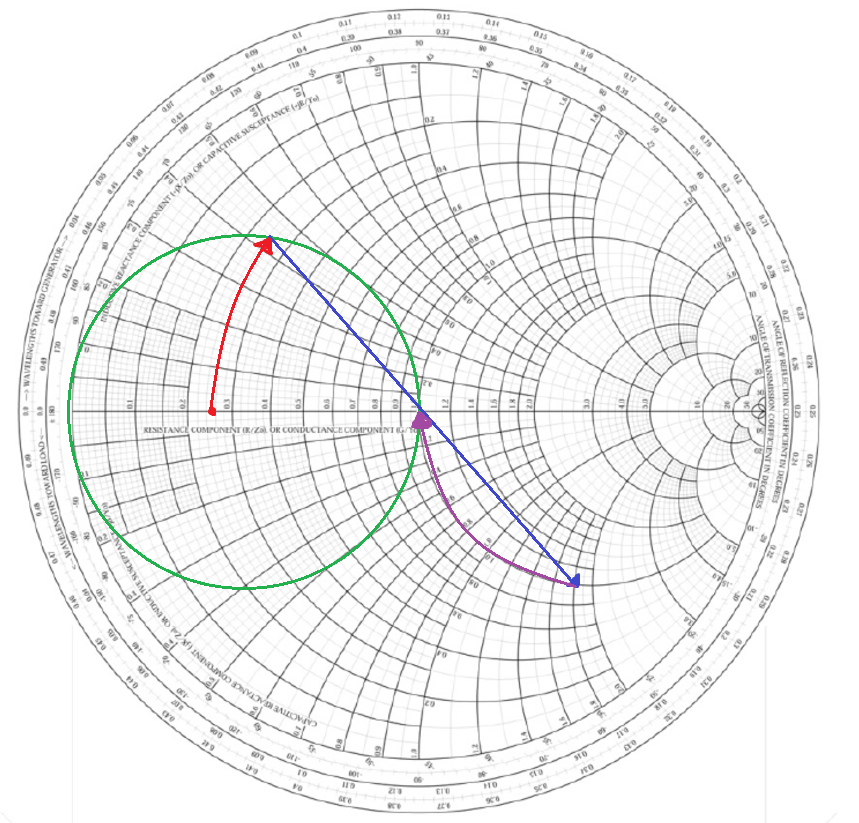
\includegraphics[width=0.7\linewidth]{figures/smith.png}
\end{center}
\end{figure}

We can travel along the constant reactance circle until we hit the big green $r = 1$ conductance circle. By moving in the clock-wise direction, we are adding capacitive susceptance, by moving counter-clockwise we are adding inductive susceptance. In either scenario, the normalized shunt susceptance is $0.44$, which we can read off using the radial constant reactance/susceptance arc values placed along the outside of the Smith Chart.

\newpage

We then switch from admittance coordinates to impedance coordinates. The $r = 1$ resistance circle is already present in the Smith Chart, and we just have to connect a line going through the center to get to this line. We can then read off which reactance arc this corresponds to to figure out how much reactance we need to add to get to the center, travelling along this line - this turns out to be around $1.8$. 



We now have our shunt admittance and series reactance components. If we want a shunt inductor, we need a corresponding series capacitor, and if we want a shunt capacitor, we need a series inductor. 
\vspace{3mm}

We first un-normalize the admittance and impedance values to get:

\[
Y = 0.0088 \;\text{S} \quad X = 90 \;\Omega
\]

\paragraph{Case 1:} 

If we want to place a shunt inductor and series capacitor, we do the following conversions:

\[
\omega L = \frac{1}{Y} \implies L \approx 18 \;\mu\text{H} \qquad
\omega C = \frac{1}{Z} \implies C \approx 1.8 \text{ nF}
\]

\paragraph{Case 2:}

If we want to place a shunt capacitor and series inductor, we do the following:

\[
\omega C = Y \implies C \approx 1.4 \text{ nF}\qquad
\omega L = Z \implies L \approx 14 \;\mu\text{H} 
\]

We place the shunt in the Y block and the impedance in the Z block. 
\vspace{3mm}

\begin{figure}[ht!]
\begin{center}
    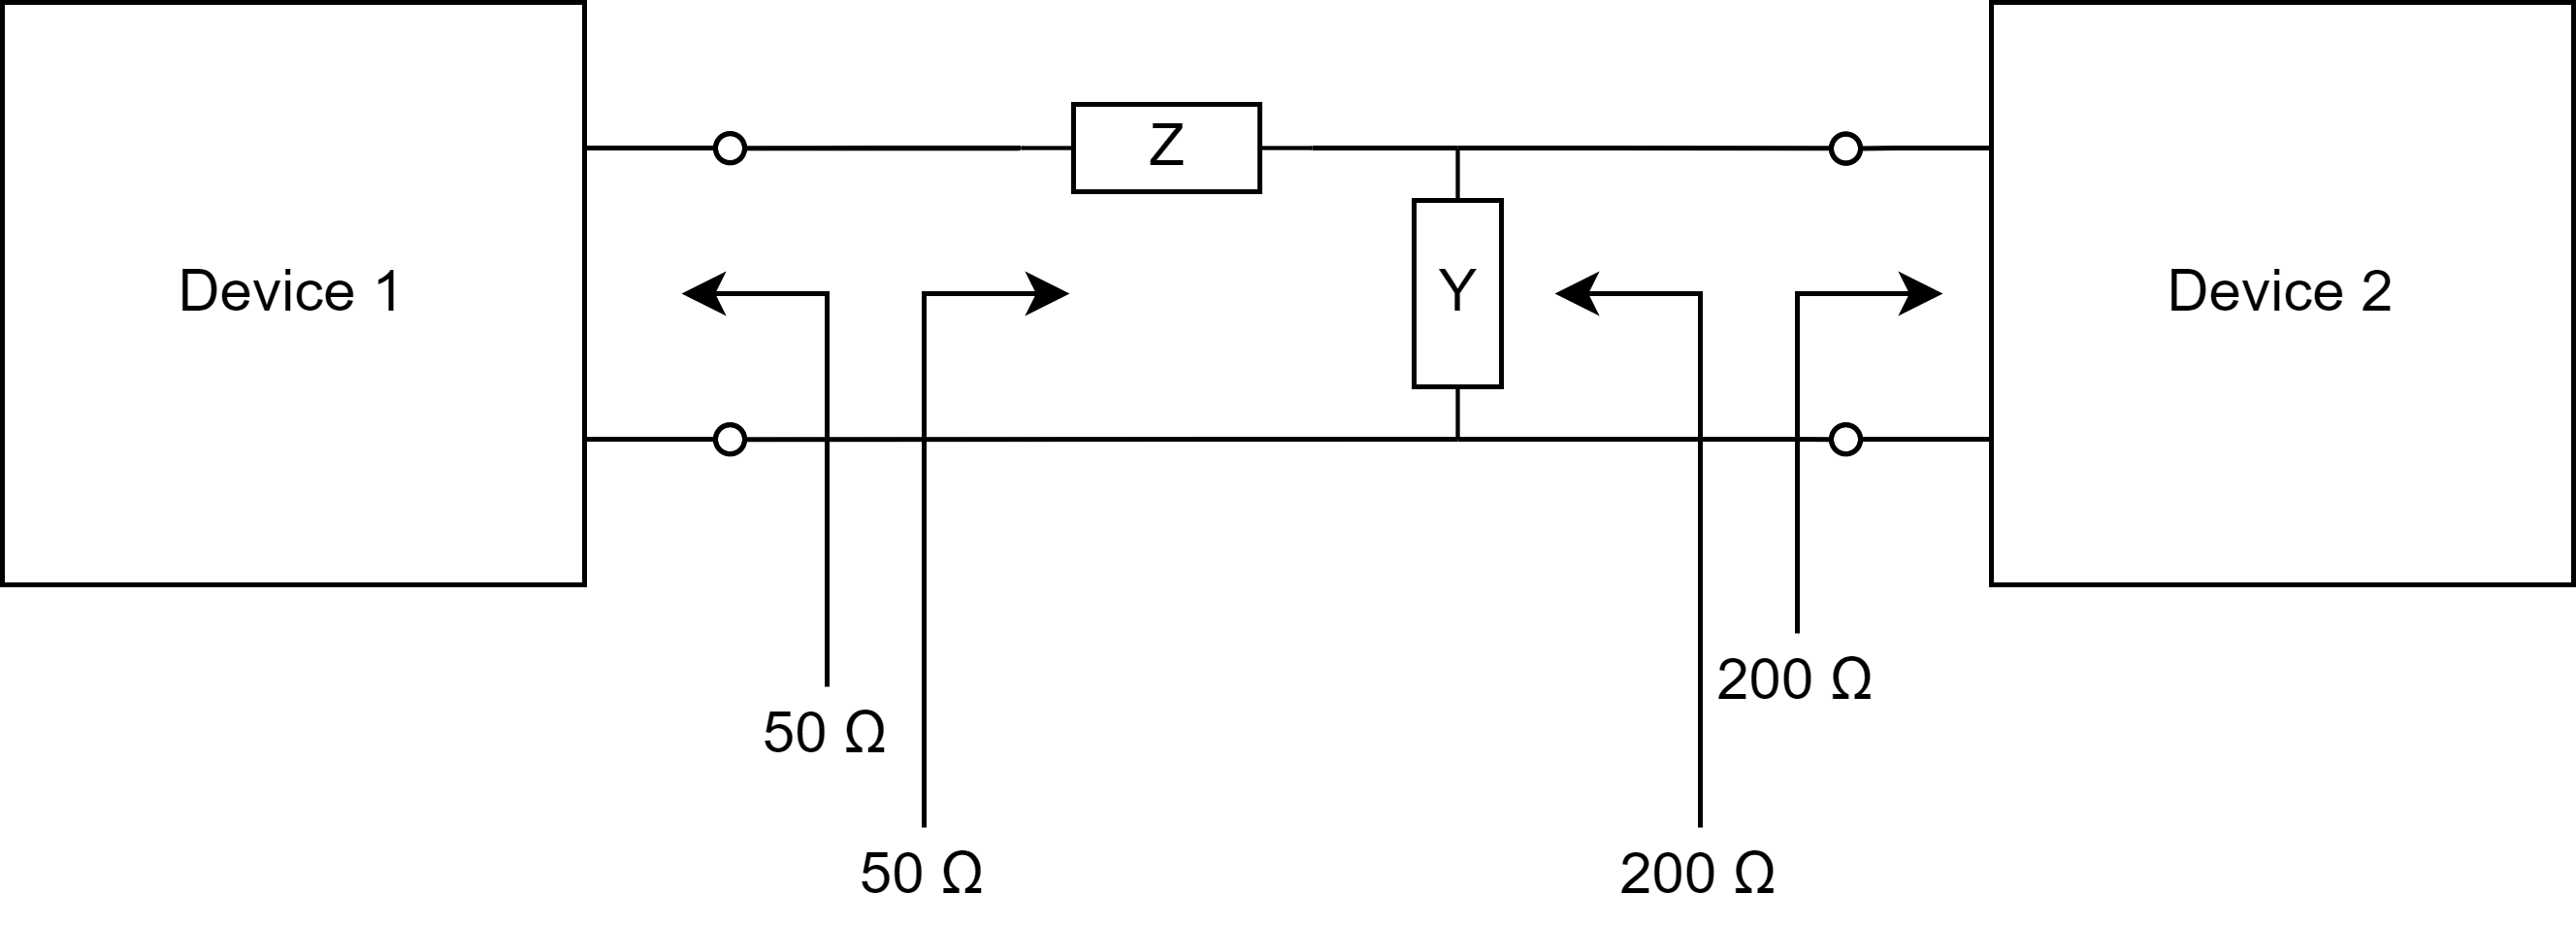
\includegraphics[width=0.7\linewidth]{figures/device.png}
\end{center}
\end{figure}

Notice how the impedance looking into each end of the network matches the impedance looking into the corresponding device terminal. This is called 'conjugate matching'. In the case where the devices exhibit a complex output impedance, the corresponding terminal must present the conjugated impedance to maximize power transfer between the device and the network and eliminate reflected voltage waves.
\vspace{3mm}

L-network matching is an alternative to stub matching. In monolithic integrated circuits, it can be very difficult or space-inefficient to create matches using stubs between different components due to area constraints. For specific frequencies, L-networks can be used to provide a small bandwidth of matched impedance. 

\end{document}
